\section{Analisi dei Dati}
La prima analisi effettuata sui dati ricavati dall'elaborazione dei risultati ottenuti da \textbf{Nicad} e \textbf{SonarQube} ha riguardato il numero di cloni sulle $4$ versioni per ogni progetto. I risultati hanno evidenziato che al crescere della versione la presenza di cloni aumenta, in particolare:
\begin{itemize}
	\item in \textbf{DnsJava}, come mostrato in \autoref{fig:nCloniDnsJava}, si hanno $146$ cloni nelle versioni $2.1.5$ e $2.1.6$, $147$ nella versione $2.1.7$ e $151$ nella $2.1.8$;
	\item in \textbf{Jabref}, come mostrato in \autoref{fig:nCloniJabRef}, si hanno $336$ nella versione $4.0$, $353$ nella $4.1$, $228$ nella $4.2$ e $357$ nella versione $4.3$;
	\item in \textbf{Fastjson}, come mostrato in \autoref{fig:nCloniFastjson}, si hanno $1107$ cloni nella versione $1.2.20$, $1230$ nella $1.2.30$ , $1292$ nella $1.2.40$ e $1358$ nella $1.2.50$.
\end{itemize}
\begin{figure}[h]
	\centering
	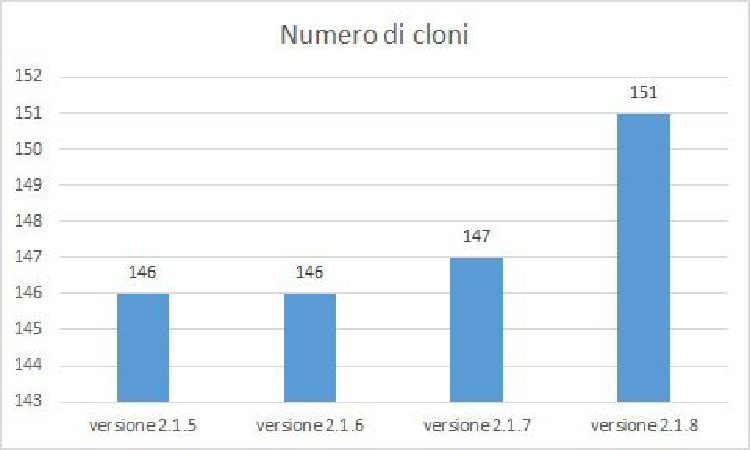
\includegraphics[scale=0.7, trim = 0cm 0cm 0cm 0cm, clip=true]{Grafici_dnsJava/NumeroCloni.pdf}
	\caption{Analisi numero cloni DnsJava}
	\label{fig:nCloniDnsJava}
	
\end{figure}
\begin{figure}[h]
	\centering
	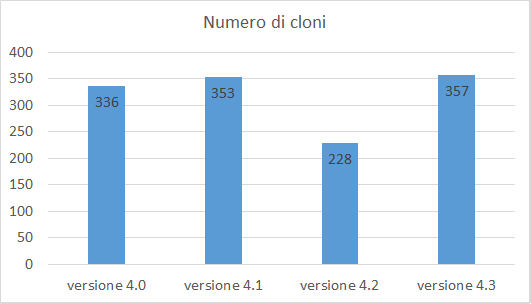
\includegraphics[scale=0.7, trim = 0cm 0cm 0cm 0cm, clip=true]{Grafici_jabRef/NumeroCloni.png}
	\caption{Analisi numero cloni JabRef}
	\label{fig:nCloniJabRef}
\end{figure}
\begin{figure}[h]
	\centering
	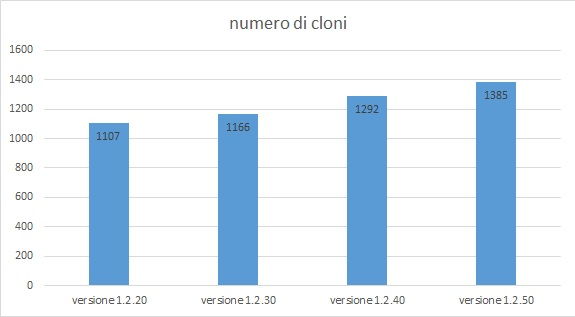
\includegraphics[scale=0.7, trim = 0cm 0cm 0cm 0cm, clip=true]{Grafici_fastJson/NumeroCloni.jpg}
	\caption{Analisi numero cloni FastJson}
	\label{fig:nCloniFastjson}
\end{figure}
Si nota dunque che l'unico dato anomalo si ha sulla versione $4.2$ di JabRef in cui il numero di cloni diminuisce rispetto alla versione precedente. Questo risultato non va però ad inficiare il trend verificato nelle analisi degli altri progetti in quanto si nota che nella versione $4.3$ vi è, non solo un aumento rispetto alla versione $4.2$, ma addirittura un incremento rispetto a tutte le precedenti versioni. 

La seconda analisi ha riguardato il \textbf{numero di cloni di ogni tipo} per le $4$ versioni di ciascuno dei progetti presi in considerazione. In linea di massima il numero di cloni di tipo $3$ è sempre maggiore rispetto ai cloni di tipo $1$ e $2$. In particolare:
\begin{itemize}
	\item in \textbf{DnsJava} si hanno:
		\begin{itemize}
				\item versione $2.1.5$: 7 cloni di tipo 1, 27 cloni di tipo 2, 112 di tipo 3;
				\item versione $2.1.6$: 7 cloni di tipo 1, 27 cloni di tipo 2, 112 di tipo 3;
				\item versione $2.1.7$: 7 cloni di tipo 1, 27 cloni di tipo 2, 113 di tipo 3;
				\item versione $2.1.8$: 9 cloni di tipo 1, 27 cloni di tipo 2, 115 di tipo 3;		
		\end{itemize}
	\item in \textbf{JabRef} si hanno:
				\begin{itemize}
			\item versione $4.0$: 8 cloni di tipo 1, 48 cloni di tipo 2,280 di tipo 3;
			\item versione $4.1$: 10 cloni di tipo 1, 49 cloni di tipo 2, 294 di tipo 3;
			\item versione $4.2$: 2 cloni di tipo 1, 20 cloni di tipo 2, 206 di tipo 3;
			\item versione $4.3$: 8 cloni di tipo 1, 49 cloni di tipo 2, 300 di tipo 3;		
		\end{itemize}
	\item in \textbf{FastJson} si hanno:
	\begin{itemize}
		\item versione $1.2.20$: 270 cloni di tipo 1, 120 cloni di tipo 2,717 di tipo 3;
		\item versione $1.2.30$: 284 cloni di tipo 1, 140 cloni di tipo 2, 742 di tipo 3;
		\item versione $1.2.40$: 301 cloni di tipo 1, 150 cloni di tipo 2, 841 di tipo 3;
		\item versione $1.2.50$: 313 cloni di tipo 1,154 cloni di tipo 2, 918 di tipo 3;		
	\end{itemize}
\end{itemize}
Quello che si nota è che in tutti i progetti analizzati il numero di cloni di tipo 3 è predominante. I cloni di tipo 2 sono maggiori rispetto a quelli di tipo 1 tranne che in FastJson essendo quest'ultima una libreria.
\begin{figure}[h]
	\centering
	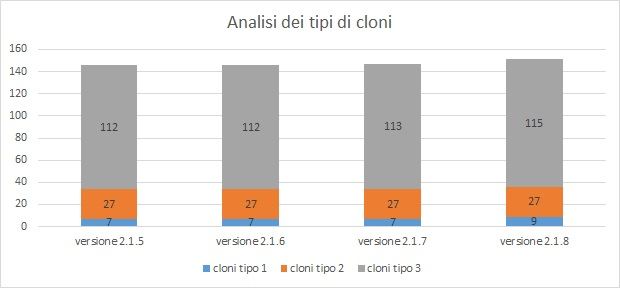
\includegraphics[scale=0.7, trim = 0cm 0cm 0cm 0cm, clip=true]{Grafici_dnsJava/TipiCloni.jpg}
	\caption{Analisi tipo cloni DnsJava}
	\label{fig:tipiCloniDnsJava}
	
\end{figure}
\begin{figure}[h]
	\centering
	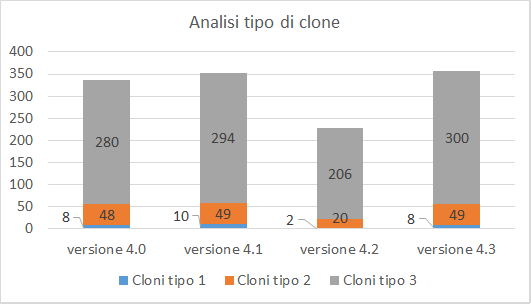
\includegraphics[scale=0.7, trim = 0cm 0cm 0cm 0cm, clip=true]{Grafici_jabRef/TipiCloni.png}
	\caption{Analisi tipo cloni JabRef}
	\label{fig:tipiCloniJabRef}
\end{figure}
\begin{figure}[h]
	\centering
	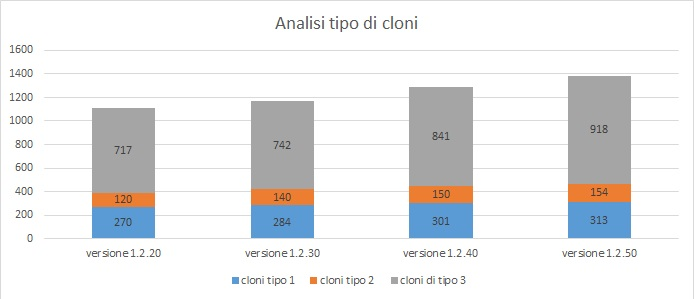
\includegraphics[scale=0.7, trim = 0cm 0cm 0cm 0cm, clip=true]{Grafici_fastJson/TipiCloni.jpg}
	\caption{Analisi tipo cloni FastJson}
	\label{fig:tipiCloniFastjson}
\end{figure}